\section{Aufbau und Durchführung}
\label{sec:Durchführung}
\subsection{Aufbau}
Zur Untersuchung des Photeffektes wird eine Photozelle genutzt, zu sehen in Abbildung \ref{fig:photozelle}.
\begin{figure}
 \centering
 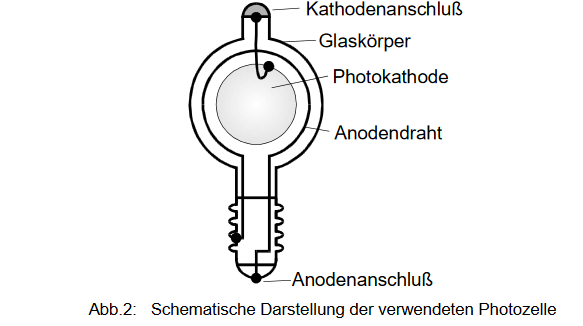
\includegraphics[width=0.7\textwidth]{photozelle.png}
 \caption{Darstellung der Photozelle.\cite{sample}}
 \label{fig:photozelle}
\end{figure}
Die Photozelle setzt sich zusammen aus einem evakuierten Glaskolben, der Photokathode und einem Drahtring der als Anode dient.
Zwischen Kathode und Anode wird eine variable Spannung angelegt und damit ein Feld erzeugt, welches die Elektronen abbremst.
Damit gelangen nur Elektronen an die Anode für die gilt:
\begin{align}
\mathrm{h}\nu=e_\mathrm{0}U_\mathrm{g}+A_\mathrm{k}.
\end{align}
Hierbei ist $e_\mathrm{0}$ die Elementarladung und $U_\mathrm{g}$ die Gegenspannung.
Der Verlauf des Photostromes ist in Abbildung $\ref{fig:ps}$ dargestellt.
\begin{figure}
 \centering
 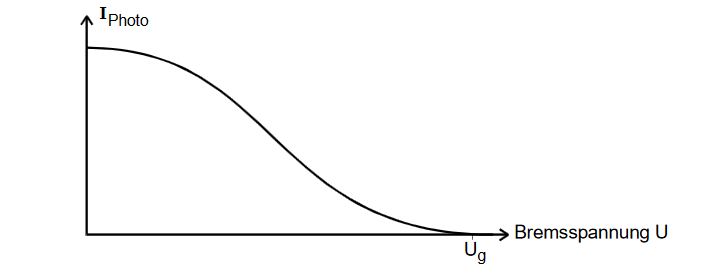
\includegraphics[width=0.7\textwidth]{ps.png}
 \caption{Der Photostrom in Abhängigkeit von der Bremsspannung.\cite{sample}}
 \label{fig:photozelle}
\end{figure}
Es lässt sich erkennen, dass der Photostrom bei bestimmten $U_\mathrm{g}$ nicht plötzlich auf null abfällt.
Dies lässt sich mit den unterschiedlichen Geschwindigkeiten der Elektronen erklären, welche bereits im Festkörper
eine gewisse Energie besitzen. Die Fermi-Dirac-Verteilung besagt, dass die Valenzelektronen eine Energie im Bereich
zwischen $0$ und $\xi$, der Fermi-Energie, besitzen.
Eine Beschleunigungsspannung muss angelegt werden, wenn die Austrittsarbeit der Anode größer als $5\nu$ ist.
Sonst müssen die Elektronen gegen ein Gegenfeld anlaufen.
Für die Messung wird der Aufbau nach Abbildung \ref{fig:optisch} genutzt.
\begin{figure}
 \centering
 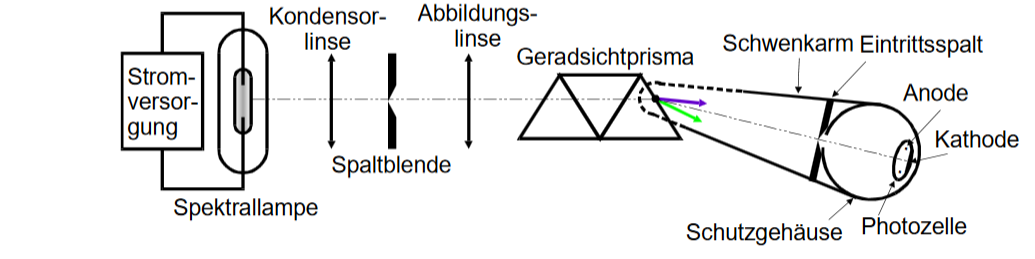
\includegraphics[width=0.7\textwidth]{aufbauganz.png}
 \caption{Gesamter Aufbau der Versuchsapparatur.\cite{sample}}
 \label{fig:optisch}
\end{figure}
Eine Spektrallampe erzeugt Licht mit bekanntem Spektrum, dies wird an der Kondensorlinse gebündelt und wandert durch
die Spaltblende und die Abbildungslinse hin zum Geradsichtprisma. Am Prisma wird das Licht in Spektrallinien aufgeteilt,
damit kann die Photozelle mit monochromatischem Licht bestrahlt werden. Ein empfindliches Strommesssgerät kann den Photostrom
messen. Die Apparatur wird nach Abbildung \ref{fig:schaltung} geschaltet.
\begin{figure}
 \centering
 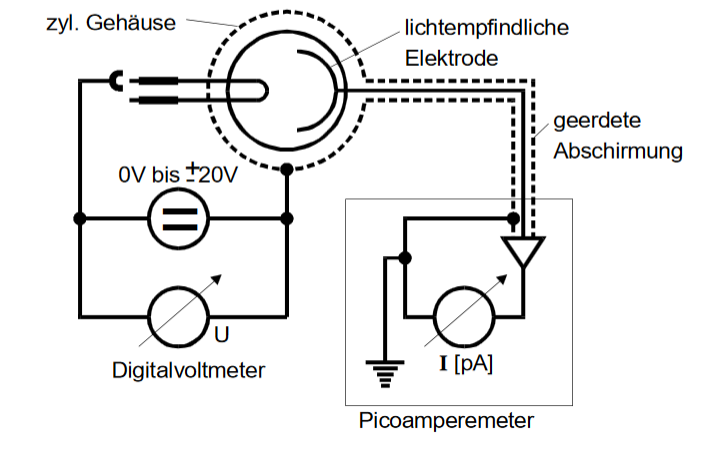
\includegraphics[width=0.7\textwidth]{schaltung.png}
 \caption{Schaltbild der Apparatur.\cite{sample}}
 \label{fig:schaltung}
\end{figure}
\subsection{Durchführung}
Die Photozelle wird verschoben, sodass eine Spektrallinie auf den Eintrittsspalt trifft.
Zu Beginn wird für fünf verschiedene, gut sichtbare Spektrallinien der Photostrom in Abhängigkeit von der Gegenspannung gemessen.
Dabei wird der Spannungsbereich betrachtet bei dem der Photostrom möglichst gering ausfällt.
Zum Schluss wird der Photostrom, in Abhängigkeit von der Spannung zwischen den beiden Elektroden, für eine Spektrallinie gemessen.
Der bemessene Spannungsbereich leigt zwischen ca. $-20-20\,\si{\volt}$ um $0\,\si{\volt}$ rum wird feinschrittiger gemessen.
